% Auriga theme
% https://github.com/anishathalye/auriga

\documentclass[14pt,aspectratio=169]{beamer}
\usepackage{pgfpages}
\usepackage{amsmath}
\usepackage{fancyvrb}
\usepackage{tikz}
\usetikzlibrary{arrows.meta, positioning, quotes}
\usepackage{pgfplots}

% \ifnotes
% \setbeamertemplate{note page}[plain]
% \setbeameroption{show notes on second screen=right}
% \fi

\usetheme{auriga}
\usecolortheme{auriga}

% define some colors for a consistent theme across slides
\definecolor{red}{RGB}{181, 23, 0}
\definecolor{blue}{RGB}{0, 118, 186}
\definecolor{gray}{RGB}{146, 146, 146}

\title{Universidad Nacional de La Plata (UNLP) \\ Maestría en Finanzas
  Públicas Provinciales y Municipales \\ La Politica de las Finanzas
  Públicas}
\subtitle{Clase 2}
\author{\underline{Sebastian Freille} \inst{1}}
\institute[IEF (FCE-UNC)]{\inst{1} Instituto de Economía y Finanzas (FCE-UNC)}
\date{}


\AtBeginSection[]{
    \begin{frame}
    \vfill
    \centering
    \begin{beamercolorbox}[sep=8pt,center,shadow=true,rounded=true]{title}
        \usebeamerfont{title}\insertsectionhead\par%
    \end{beamercolorbox}
    \vfill
    \end{frame}
}

%\addtobeamertemplate{headline}{}{\rule{\paperwidth}{1pt}}


\begin{document}
\maketitle


\section{Modelizacion del problema de la política económica}


  \begin{frame}\frametitle{Introducción}
    \begin{itemize}\itemsep 10pt
    \item Elección de la política económica importa una decisión
      colectiva a partir de intereses (preferencias) individuales e
      instituciones políticas determinadas
      \item Decisiones difieren según instituciones políticas
        --dictadura versus democracia $\longrightarrow$ tanto en el
        proceso como en los resultados
       \item Existen dos modelos tipicos de democracia --directa y
         representativa. Si bien difieren en muchos aspectos, ambas
         tienen en el centro del proceso decisorio a mecanismos de
         votacion. 
      \end{itemize}
    \end{frame}



    \begin{frame}\frametitle{Un modelo simple}
    \begin{itemize}\itemsep 10pt
    \item Individuos maximizan una función de utilidad
      $U(x_{1},x_{2};\alpha^{i})$ --$x_{1}$ y $x_{2}$ bienes
      privados. El gobierno le saca $\tau$ del $Y$ al individuo y le
      devuelve $T$ como transferencia de suma fija.
      \begin{equation*}
        p_{1}x_{1}+p_{2}x_{2} \leq (1-\tau)Y+T
      \end{equation*}
      \item El problema consiste en maximizar la utilidad sujeta a la
        restricción presupuestaria $\longrightarrow$ se obtienen las
        demandas individuales $x_{1}(p_{1},p_{2},Y,\tau,T;\alpha^{i})$
        y $x_{2}(p_{1},p_{2},Y,\tau,T;\alpha^{i})$
        \item El parámetro $\alpha$ en la función de utilidad captura
          la heterogeneidad de preferencias.
      \end{itemize}
    \end{frame}


    \begin{frame}\frametitle{Un modelo simple (cont.)}
    \begin{itemize}\itemsep 10pt
    \item Reemplazando esas demandas en la función de utilidad, se
      obtiene la funcion de utilidad indirecta:
      \begin{align*}
        V(p_{1},p_{2},Y,,\tau,T;\alpha^{i}) \equiv \\
        U(x_{1}(p_{1},p_{2},Y,\tau,T;\alpha^{i}),x_{2}(p_{1},p_{2},Y,\tau,T;\alpha^{i});\alpha^{i})
      \end{align*}
      \item Importante $\longrightarrow$ utilidad es función de las
        variables de política [dado que $x_{1}$ y $x_{2}$ son elegidos
        de manera óptima]
        \begin{align*}
V(\tau,T;\alpha^´{i}) \equiv \\ V(p_{1}(\tau,T),p_{2}(\tau,T),Y(\tau,T),\tau,T;\alpha^{i})
          \end{align*}
      \end{itemize}
    \end{frame}
    

   \begin{frame}\frametitle{Un modelo simple (cont.)}
    \begin{itemize}\itemsep 10pt
    \item Conociendo $\tau$ conocemos $T$ [¿por qué?] y la fn UI:
      \begin{equation*}
V(\tau;\alpha^{i})
\end{equation*}
\item La política preferida por el individuo se obtiene hallando $\tau$
  que maximiza utilidad indirecta:
  \begin{equation*}
\frac{\partial V(\tau;\alpha^{i})}{\partial \tau}=0
\end{equation*}
\item  $\tau^{*}(\alpha^{i})$ $\longrightarrow$
  dimensión política evidente --$\alpha^{i}$'s diferentes implican
  políticas (alícuotas) preferidas diferentes
      \end{itemize}
    \end{frame}
    


    
\section{Racionalidad, preferencias y decisiones colectivas}


  \begin{frame}\frametitle{¿Cómo se decide el nivel de gasto público?}
    \begin{itemize}
    \item El nivel de gasto en bienes y servicios públicos (y de
      impuestos) se decide a través del proceso político --a
      diferencia del gasto en bienes privados
      \item Los ciudadanos eligen a representantes por medio de algún
        sistema de votación, los cuales votan a su vez un presupuesto
        público que contiene un determinado nivel de gastos e ingresos
        \item Cuando un legislador vota, debe decidir sobre dos cosas:
          1) averiguar los puntos de vista de sus electores; 2)
          decidir que peso asignar a intereses (potencialmente) divergentes
      \end{itemize}
    \end{frame}

    

\begin{frame}\frametitle{}
  \begin{block}{Racionalidad}
Los individuos que nos interesa estudiar son personas comunes que
tienen \textbf{deseos} y \textbf{creencias}. Ambos afectan su
comportamiento. Hay \textbf{deseos} que provienen desde la propia naturaleza
humana como el deseo de supervivencia y reproducción, otros que
provienen de la vida social, como el tipo de ropa que usamos o la música
que escuchamos y otros que provienen de fuentes religiosas, culturales
ideológicas, entre otras. En el mundo de la economía política, nos referimos a
los deseos como \textbf{preferencias}. Y no nos interesa explicar por
qué las preferencias son como son --son \textit{dadas} y
\textit{estables}, sino que nos preocupa analizar el impacto de esas preferencias. 
    \end{block}
  \end{frame}


\begin{frame}\frametitle{Preferencias}
  \begin{itemize}
    \item El mundo de las preferencias es un \textit{mundo interior}
    $\longrightarrow$ las personas no revelan en todo momento y lugar
    sus preferencias sobre todas las cosas.
    \item Debemos hacer algunos
    \textit{supuestos} sobre sus preferencias --pueden derivarse de
    intuiciones, evidencias.
    \item Pero también existe un \textit{entorno exterior}
      $\longrightarrow$ incertidumbre de diversa indole. Esta
      incertidumbre \textit{afecta} la forma en que los individuos
      expresan sus preferencias.  
    \end{itemize}
  \end{frame}
  

  \begin{frame}\frametitle{}
  \begin{block}{Incertidumbre, preferencias y comportamiento}
Supongamos que mi \textit{preferencia} sea obtener
un 10 en el examen. Yo no puedo elegir ``obtener un 10 en
el examen''. Pero puedo elegir un \textit{instrumento} (acción) para
llegar a obtener un \textit{resultado} en línea con mi preferencia. Si una acción es ``estudiar la noche
previa'' y la otra es ``ir al cine la noche previa'' y si se sabe con
certeza que la primera conducirá al resultado preferido, entonces como
actor racional elijo aquella que conduzca al resultado. \underline{PERO:} en
general los individuos no tienen conocimiento perfecto de como un
instrumento conduce al resultado. Además, eventos inesperados. Es aquí donde entran las \textbf{creencias}
    \end{block}
  \end{frame}


  
\begin{frame}\frametitle{Creencias}
  \begin{itemize}
    \item \textbf{Creencias} $\longrightarrow$ ideas que un individuo
      posee en relación a la eficacia de un determinado instrumento
      (comportamiento o acción) para obtener un resultado que está en
      línea con un \textbf{deseo} de ese individuo.
      \item Las \textbf{creencias} conectan los instrumentos con los
        resultados. Cuando un individuo actua de acuerdo tanto en base
        a sus preferencias como a sus creencias, se dice que existe
        \textbf{racionalidad instrumental}.
        \item Las \textbf{creencias} cambian y eso hace que se revisen las ideas sobre la
          eficacia de los instrumentos. 
    \end{itemize}
  \end{frame}


  \begin{frame}\frametitle{Resumiendo}
  \begin{block}{Elección racional: Preferencias y creencias}
Un \textbf{individuo racional} es aquel que combina
 \textbf{creencias} sobre el \textbf{entorno exterior} y
 \textbf{preferencias} sobre \textbf{cosas del entorno exterior} de
 una manera consistente. Este enfoque implica una forma de
 \textbf{individualismo metodológico}. Lo más relevante de este
 enfoque es la observación de que los \textbf{individuos} tienen
 preferencias y creencias. Los colectivos --grupos, clases, empresas,
 naciones- no tienen preferencias y creencias en el sentido
 cognitivo. Aquí entra en juego el tema de la \textbf{agregación de
   preferencias y creencias}    \end{block}
  \end{frame}
  


  \begin{frame}\frametitle{Preferencia y elección}
  \begin{itemize}
    \item Un individuo, $i$, y tres objetos --''alternativas''-, $A$, $B$, y $C$
      sobre los cuales $i$ tiene preferencias.
      \item El individuo $i$ es capaz de hacer evaluaciones
        del tipo:
        \begin{itemize}\itemsep 5pt \smallskip
        \item ``Prefiero $A$ a $B$''
          \item ``Soy indiferente entre $B$ y $C$''. 
          \end{itemize}
          \item La relación $A \succ B$ representa en simbolos el
            primer enunciado; la relación $B ~ C$ el segundo
            \item La \textbf{elección} de $i$ es racional
              si está de acuerdo con su \textbf{preferencia}. 
            \end{itemize}
  \end{frame}


\begin{frame}\frametitle{Propiedades de las relaciones de preferencia}
\begin{block}{Completitud (comparabilidad)}
Las alternativas son comparables si,
dadas dos alternativas posibles, $A$ y $B$, tenemos ya sea $A \succ
B$, $B \succ A$, o $A ~ B$. Las alternativas son comparables si,
dado cualquier par, el individuo $i$ prefiere la primera a la
segunda, la segunda a la primera, o es indiferente entre una y otra.
\end{block}
\begin{block}{Transitividad}
La relación de preferencia es transitiva si,
dadas tres alternativas --$A$, $B$, y $C$-, si $A \succ B$ y $B \succ
C$, entonces $A \succ C$. Si el individuo $i$ prefiere $A$ a $B$ y $B$ a $C$, entonces prefiere $A$ a $C$.
\end{block}
\end{frame}



\begin{frame}\frametitle{Ordenamiento de preferencias}
\begin{itemize}
\item Si las preferencias de $i$ satisfacen estas propiedades, se dice
  que $i$ tiene un \textbf{ordenamiento de preferencias}. La elección
  racional será aquella que esté al inicio (a la iquierda) del
  ordenamiento
\item Estos ordenamientos de preferencias son
  \textbf{personales}. Cada persona puede tener un ordenamiento
  diferente. 
\item No todas las relaciones entre ``alternativas'' son
  \textbf{completas} o \textbf{transitivas}. Ejemplos:
\begin{itemize}\itemsep 5pt \smallskip
\item La comparación debe tener sentido para el individuo
  $\longrightarrow$ elegir entre cosas desconocidas (comparabilidad);
  además, la comparación debe ser sobre algo que le importa al individuo
\end{itemize}
\end{itemize}
\end{frame}


\begin{frame}\frametitle{Ejemplo: Preferencias deportivas}
\begin{itemize}
\item Supongamos que le pedimos a un ciudadano que elabore su relación de
  preferencias por los equipos del Mundial 2018. En total son 32
  equipos. 
\item Si esta persona sólo tiene algun tipo de información sobre 31 de
  los 32 equipos --desconoce absolutamente todo sobre Islandia
  $\longrightarrow$ viola propiedad de ``completitud''
  \item Si esta persona puede comparar todos los equipos en su
    deseo de quien le gustaría gane el Mundial y los ordena así: $Ger
    \succ Bra$ y $Bra \succ Uru$, pero prefiere que $Uru \succ Ger$
    $\longrightarrow$ viola propiedad de ``transitividad''. 
\end{itemize}
\end{frame}

\section{Agregación de preferencias individuales}


\begin{frame}
\frametitle{De la elección individual a la elección social}
\begin{itemize}
\item Teoría de la elección social  $\longrightarrow$ estudio de los
  procesos colectivos de decisión a través de modelos de cómo agregar insumos individuales --preferencias, bienestar- en productos colectivos --preferencias, bienestar.
\item Condorcet y  Borda plantearon el
  problema en el siglo 19; Arrow, Sen y Black lo teorizaron en el
  siglo 20.
\item La influencia de la teoría de la elección social ha sido
  fundamental en el progreso de la economía, la ciencia política y la
  sociología, entre otras disciplinas
\end{itemize}
\end{frame}


% \begin{frame}\frametitle{Ilustración: ¿Por qué vota la gente?}
%       \begin{block}{Los motivos del voto}
% En muchas elecciones las tasas de participación son relativamente
% bajas y/o vienen disminuyendo. Desde un punto de vista puramente
% económico, los beneficios de votar para un individuo son bajos (pocas
% chances de influir en el resultado). Y los costos de votar
% --levantarse temprano, movilidad, etc- suelen ser altos. El tema es
% que la probabilidad que tiene una persona de influir sobre el
% resultado electoral es virtualmente nula. Sin embargo, la gente si
% vota. En Argentina, lo hace porque es obligatorio, entre otras
% cosas. En EEUU, lo hace porque le interesa. Pero en general la gente
% vota porque le da utilidad o satisfacción (deber cívico). 
%         \end{block}
%       \end{frame}


     %  \begin{frame}\frametitle{Participación y voto: Evidencia}
 % \begin{figure}[htbp]\vspace{-2.5cm}
 %    \centering
 %    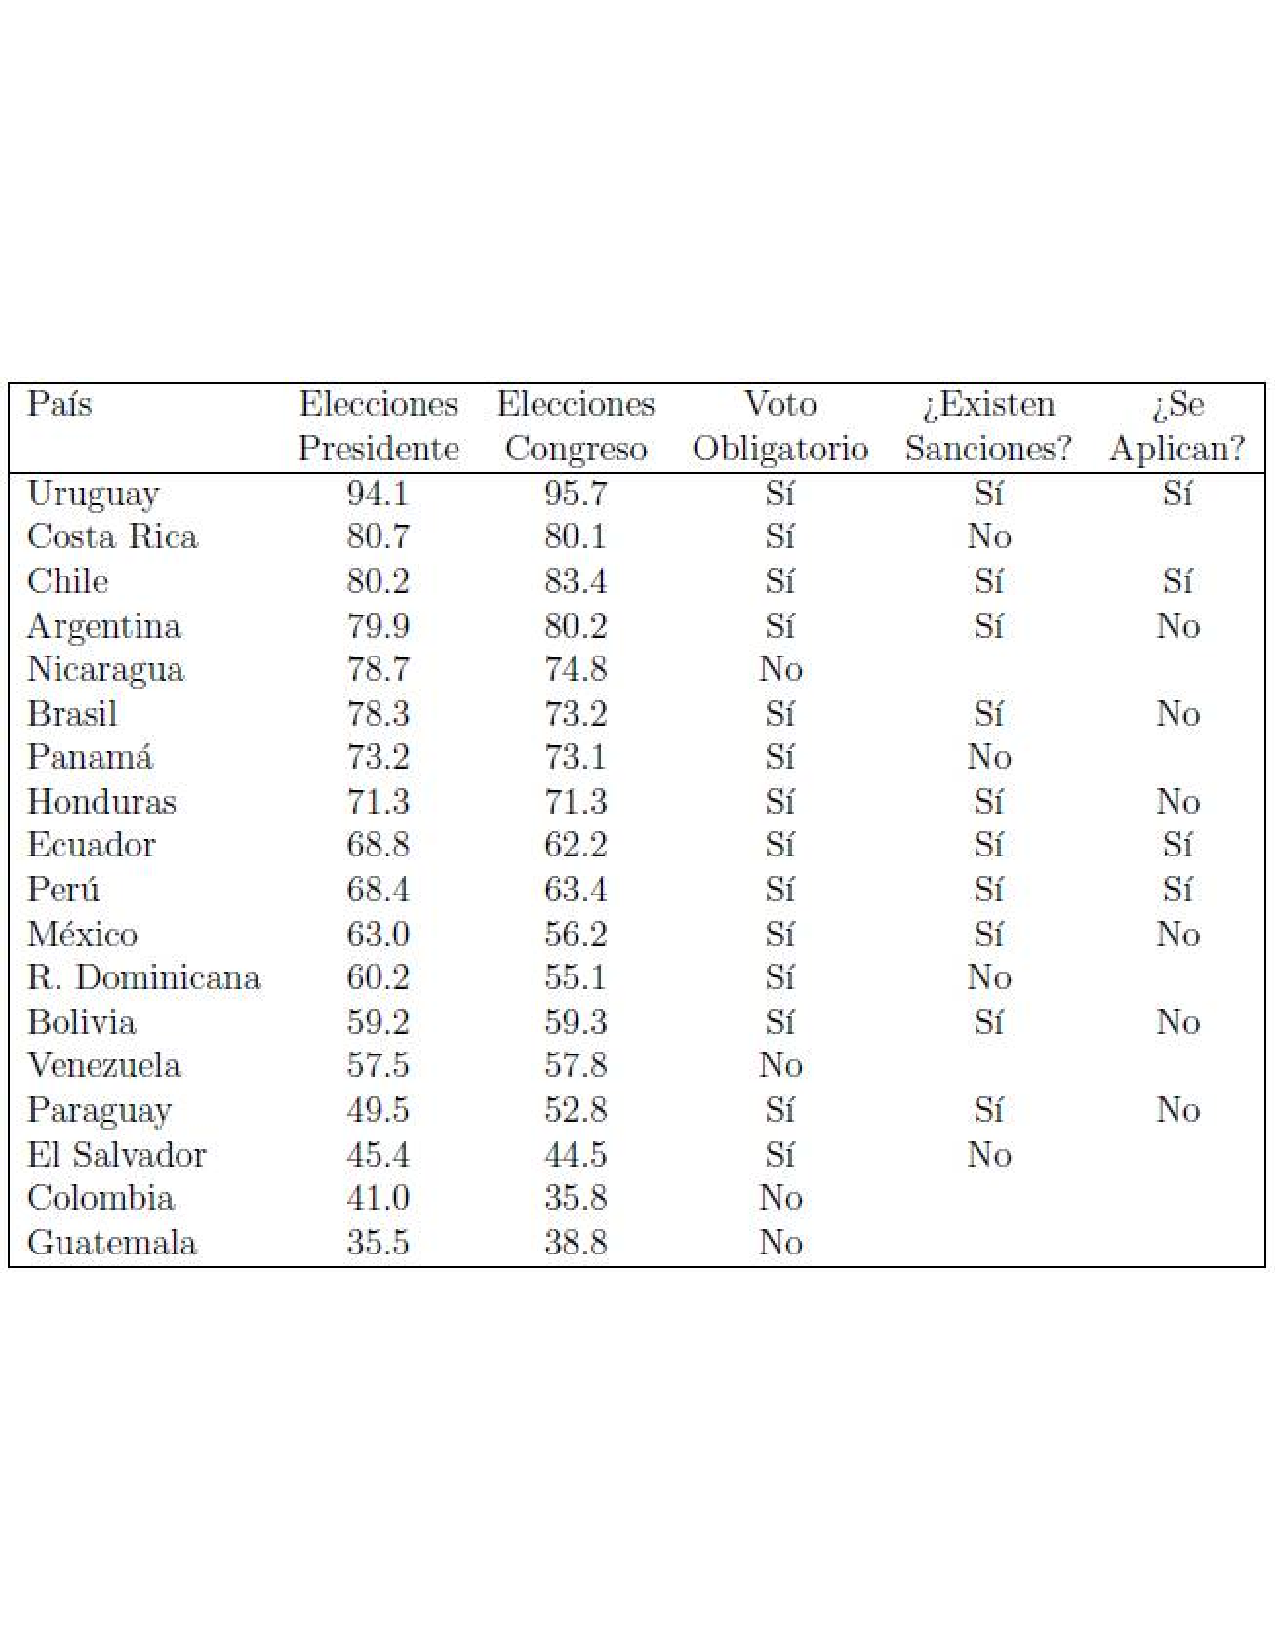
\includegraphics[scale=0.45]{uni2_turnout}
 %    \caption{Participación electoral en AL}
 %    \label{fig:1}
 %  \end{figure}
 %        \end{frame}


\begin{frame}\frametitle{Supuestos del análisis posterior}
  \begin{itemize}
  \item Existe un \textbf{número impar de individuos} que eligen
    entre:
    \begin{itemize}\itemsep 10pt \medskip
    \item Dos (2) alternativas
    \item Más de dos (2) alternativas
    \end{itemize}
  \item Los individuos eligen \textbf{racionalmente}
    \item Los individuos votan \textbf{sinceramente} --no
      estrategicamente
      \item Todos los individuos \textbf{participan}. 
    \end{itemize}
  \end{frame}

  \begin{frame}\frametitle{Reglas de decisión/elección}
    \begin{itemize}
    \item Existen múltiples reglas de votación:
      \begin{itemize}\itemsep 10pt \medskip
      \item Unanimidad $\longrightarrow$ \textbf{todos} tienen que
        preferir la misma alternativa
        \item Regla de mayoría de primera preferencia
          $\longrightarrow$ todos eligen su primera preferencia y si
          alguna recibe la mitad mas uno de los votos, es la elegida.
          \item Regla de mayoría con votación round-robin
            $\longrightarrow$ se combinan las alternativas en todos
            los pares posibles y se votan en rondas.
            \item Regla de mayoría con fijación de agenda
              $\longrightarrow$ se vota de a pares pero alguien fija
              la agenda
          \end{itemize}
          \item Nos concentramos en regla de mayoría con round-robin. 
      \end{itemize}
    \end{frame}

  
\begin{frame}\frametitle{Dos alternativas}
\begin{itemize}
\item Condiciones deseadas de un sistema de reglas de votación entre dos
  alternativas:
\begin{itemize}
\item \textbf{Anonimidad} $\longrightarrow$ si dos votantes cambian sus votos
  antes de emitirlos, el resultado de la elección no cambia (votantes
  tratados simétricamente)
\item \textbf{Neutralidad} $\longrightarrow$ si una nueva elección se hace y
  cada votante individual revierte su orden de preferencia --i.e si
  originalmente votó por A, ahora lo hace por B y viceversa-, el
  resultado de la elección se revierte (alternativas tratadas simétricamente)
\item \textbf{Monotonicidad} $\longrightarrow$ si se hace una nueva elección y
  un votante único que originalmente votó por el perdedor de la
  elección y ahora vota por el ganador, el ganador de la elección
  sigue siendo el mismo.
\end{itemize}
\end{itemize}
\end{frame}



\begin{frame}\frametitle{Dos alternativas (cont.)}
\begin{itemize}
\item Caso de dos opciones $\longrightarrow$ siempre que el número de votantes sea impar, habrá un resultado cierto. Si se vota por regla de mayoría, se elegirá la opción preferida por una mayoría de votantes, i.e. $ \frac{N+1}{2} $
\end{itemize}
\begin{block}{Teorema de May}
El único método que satisface las condiciones de anonimidad,
neutralidad y monotonicidad para determinar un
ganador de una elección entre dos alternativas es la regla de la
mayoría.
\end{block}
\end{frame}


\begin{frame}\frametitle{Dos alternativas: Ejemplo}
\begin{block}{Tres votantes, dos alternativas}
Suponga que:
\begin{enumerate}
\item $A \succ B$
\item $A \succ B$
\item $B \succ A$
\end{enumerate}
\item El ganador por mayoría simple de esta elección es $A$.
¿Que pasa si dos votantes intercambian sus votos? (anonimidad)
\begin{enumerate}
\item $A \succ B$
\item $B \succ A$
\item $A \succ B$
\end{enumerate}
\end{block}
\end{frame}


\begin{frame}\frametitle{Dos alternativas: Ejemplo (cont.)}
\begin{block}{Tres votantes, dos alternativas}
¿Que pasa si cada uno revierte su preferencia? (neutralidad)
\begin{enumerate}
\item $B \succ A$
\item $B \succ A$
\item $A \succ B$
\end{enumerate}
¿Qué pasa si 3 ahora
vota por el ganador? (monotonicidad)
\begin{enumerate}
\item $A \succ B$
\item $A \succ B$
\item $A \succ B$
\end{enumerate}
El ganador sigue siendo el mismo, $A$.
\end{block}
\end{frame}


% \begin{frame}\frametitle{Ejercicio}
% \begin{block}{Ejercicio}
% Considere los siguientes sistemas para elegir el ganador de una
% elección entre dos alternativas y determine cuáles de las tres
% condiciones son satisfechas y cuales no.
% \begin{itemize}
% \item dictadura $\longrightarrow$ todos votan, pero sólo cuenta el
%   voto del dictador
% \item regla impuesta $\longrightarrow$ un candidato gana
%   independientemente de los votos emitidos
% \item ``pariah'' $\longrightarrow$ un votante especial denominado
%   ``pariah''; se ignora su voto; el ganador decido usando mayoría
%   simple para resto de votos
% \item

% \end{itemize}
% \end{block}
% \end{frame}


\section{Paradoja de Condorcet y Teorema de Imposibilidad}

\begin{frame}\frametitle{Más de dos alternativas}
\begin{itemize}
\item Con dos alternativas $\longrightarrow$ regla de mayoría para
  agregar preferencias individuales en preferencias sociales produce
  un claro ganador que satisface propiedades deseadas (siempre que
  número de votantes sea impar)
\item ¿Qué sucede si, como en innumerables situaciones de la vida
  real, hay más de dos alternativas?
\item El problema se vuelve más complejo. Problema $\longrightarrow$
  existe alguna regla de votación que permita agregar preferencias
  individuales en preferencias sociales y que produzca un claro
  ganador y que satisfaga propiedades deseadas?
\begin{itemize}\itemsep 5pt \medskip
\item La respuesta es \textbf{no}.
\end{itemize}
\end{itemize}
\end{frame}


\begin{frame}\frametitle{Condorcet: Teorema y paradoja}
\begin{block}{Teorema del jurado de Condorcet}
Si cada miembro de un jurado tiene una probabilidad igual e
independiente, $0.5<p<1$ de adoptar la decisión correcta sobre la
culpabilidad o inocencia de un acusado, entonces la probabilidad de
que el jurado como un todo adopte la decisión correcta se acercará a 1
a medida que el tamaño aumenta.
\end{block}
\begin{block}{La paradoja de Condorcet}
A pesar de que las preferencias individuales sean ``racionales''
(transitivas), las preferencias del grupo (mayoría) pueden ser
``irracionales'' (no transitivas). 
\end{block}
\end{frame}

\begin{frame}\frametitle{La solución y el problema}
\begin{itemize}
\item La primera idea de Condorcet permite permite justificar
  votaciones colectivas que incluyan, dentro de lo posible, el mayor
  tamaño posible de grupo --jurados populares, elecciones
  presidenciales.
\item La segunda idea plantea un problema en relación al metódo de
  decisión colectiva $\longrightarrow$ la elección por mayoría simple
  es un método válido de elección pero puede estar asociado a este
  problema de ``irracionalidad'' del colectivo.
\item Sus planteos le valieron conceptos actuales como \textit{ganador
    de Condorcet} y \textit{ciclos de Condorcet}.
\end{itemize}
\end{frame}


\begin{frame}\frametitle{La paradoja de Condorcet: Ilustración}
\begin{itemize}
\item Suponga que un colectivo debe elegir entre tres alternativas: A, B y
  C. Se pueden imaginar 6 formas diferentes en que las
  preferencias pueden ser ordenadas:
\begin{itemize}
\item $A \succ B \succ C$
\item $A \succ C \succ B$
\item $B \succ A \succ C$
\item $B \succ C \succ A$
\item $C \succ A \succ B$
\item $C \succ B \succ A$
\end{itemize}
\item Suponga ahora que el colectivo está compuesto por sólo 3
  individuos cuyas preferencias son:
\end{itemize}
\end{frame}


\begin{frame}\frametitle{La paradoja de Condorcet: Ilustración (cont.)}
\begin{enumerate}\itemsep 5pt
\item $A \succ B \succ C$
\item $B \succ C \succ A$
\item $C \succ A \succ B$
\end{enumerate}
\begin{itemize}
\item Imagine ahora que se vota de a pares.
\begin{itemize}\itemsep 5pt
\item Supongamos un voto entre A y B. ¿Quién gana? A
\item Supongamos un voto entre B y C. ¿Quién gana? B
\item Supongamos un voto entre C y A. ¿Quién gana? C
\end{itemize}
\item ¿Qué alternativa debería ganar si hay transitividad?
  A. \textbf{Pero} no hay transitividad. Se da un \textit{ciclo de
    Condorcet}
\begin{equation*}
A \succ B \succ C \succ A
\end{equation*}
\end{itemize}
\end{frame}

\begin{frame}\frametitle{Ciclos de Condorcet y ganadores de Condorcet}
\begin{block}{Ganador de Condorcet}
Un \textit{ganador de Condorcet} es una alternativa tal que recibe la
mayoría de los votos cuando es apareada contra cada una de las otras alternativas
\end{block}
\bigskip
\begin{block}{Ciclos de Condorcet}
Un \textit{ciclo de Condorcet} ocurre cuando existe una violación del
principio de transitividad en el ordenamiento de las preferencias sociales
\end{block}
\end{frame}


\begin{frame}\frametitle{Ciclos de Condorcet y ganadores de Condorcet}
\begin{block}{Teorema I}
Si hay un ciclo de Condorcet, no hay ganador de Condorcet
\end{block}
\begin{block}{Ejemplo}
Consideremos el caso con tres alternativas. Sea $A \succ B \succ C
\succ A$. ¿Es A un ganador de Condorcet? $\longrightarrow$ No, dado que $C
\succ A$. ¿Algún otro (B o C) es un ganador de Condorcet? $\longrightarrow$
 No, porque $A \succ B$ (B no es). No, porque $B \succ C$ (C no es)
\end{block}
\begin{block}{Teorema II}
Hay ciclo de Condorcet cuando no hay ganador de Condorcet
\end{block}
\end{frame}

\begin{frame}\frametitle{Relevancia de los ciclos de Condorcet}
\begin{itemize}
\item La existencia de ciclos de Condorcet implica que \textit{el
    orden en que se vota es crucial}
\item Recordando las preferencias que generaron un ciclo de
  Condorcet. Supongamos que el orden de votación es:
\begin{itemize}\itemsep 5pt \smallskip
\item 1ra votación: A vs B. 2da votación: ganador de A vs B
  contra C
\begin{itemize}\itemsep 5pt \smallskip
\item Dado que $A \succ B$ y $C \succ A$, \underline{gana C}
\end{itemize}
\item 1ra votación: A vs C. 2da votación: ganador de A vs C
  contra B.
\begin{itemize}\itemsep 5pt \smallskip
\item Dado que $C \succ A$ y $B \succ C$, \underline{gana B}
\end{itemize}
\item 1ra votación: B vs C. 2da votación: ganador de B vs C contra A.
\begin{itemize}\itemsep 5pt \smallskip
\item Dado que $B \succ C$ y $A \succ B$, \underline{gana A}.
\end{itemize}
\end{itemize}
\item La alternativa electa depende de cómo (y quién) se disponga el orden de votación!
\end{itemize}
\end{frame}

\begin{frame}\frametitle{Implicancias para votaciones: Agenda-setting}
\begin{itemize}
\item Este simple ejemplo ilustra la importancia decisiva del ``poder de
  agenda'' --qué alternativas considerar y en qué orden las
  consideramos y votamos.
\item ¿Quiénes establecen la agenda en la vida real?
\begin{itemize}\itemsep 5pt \medskip
\item En el Congreso, el Presidente de la Cámara y los Presidentes de
  Comisión tienen amplios poderes para decidir que asuntos se giran y
  para proponer el orden de votaciones en el recinto. En EEUU, es el
  Speaker of the House y el Senate Majority Leader
\item En regímenes presidencialistas, los ejecutivos también tienen
  poder de agenda (DNU, vetos, poderes delegados)
\end{itemize}
\item El poder de agenda no es ilimitado ni da control absoluto
\end{itemize}
\end{frame}

\begin{frame}\frametitle{¿Son relevantes en la práctica estos ciclos?}
  \begin{figure}[htbp]
    \centering
    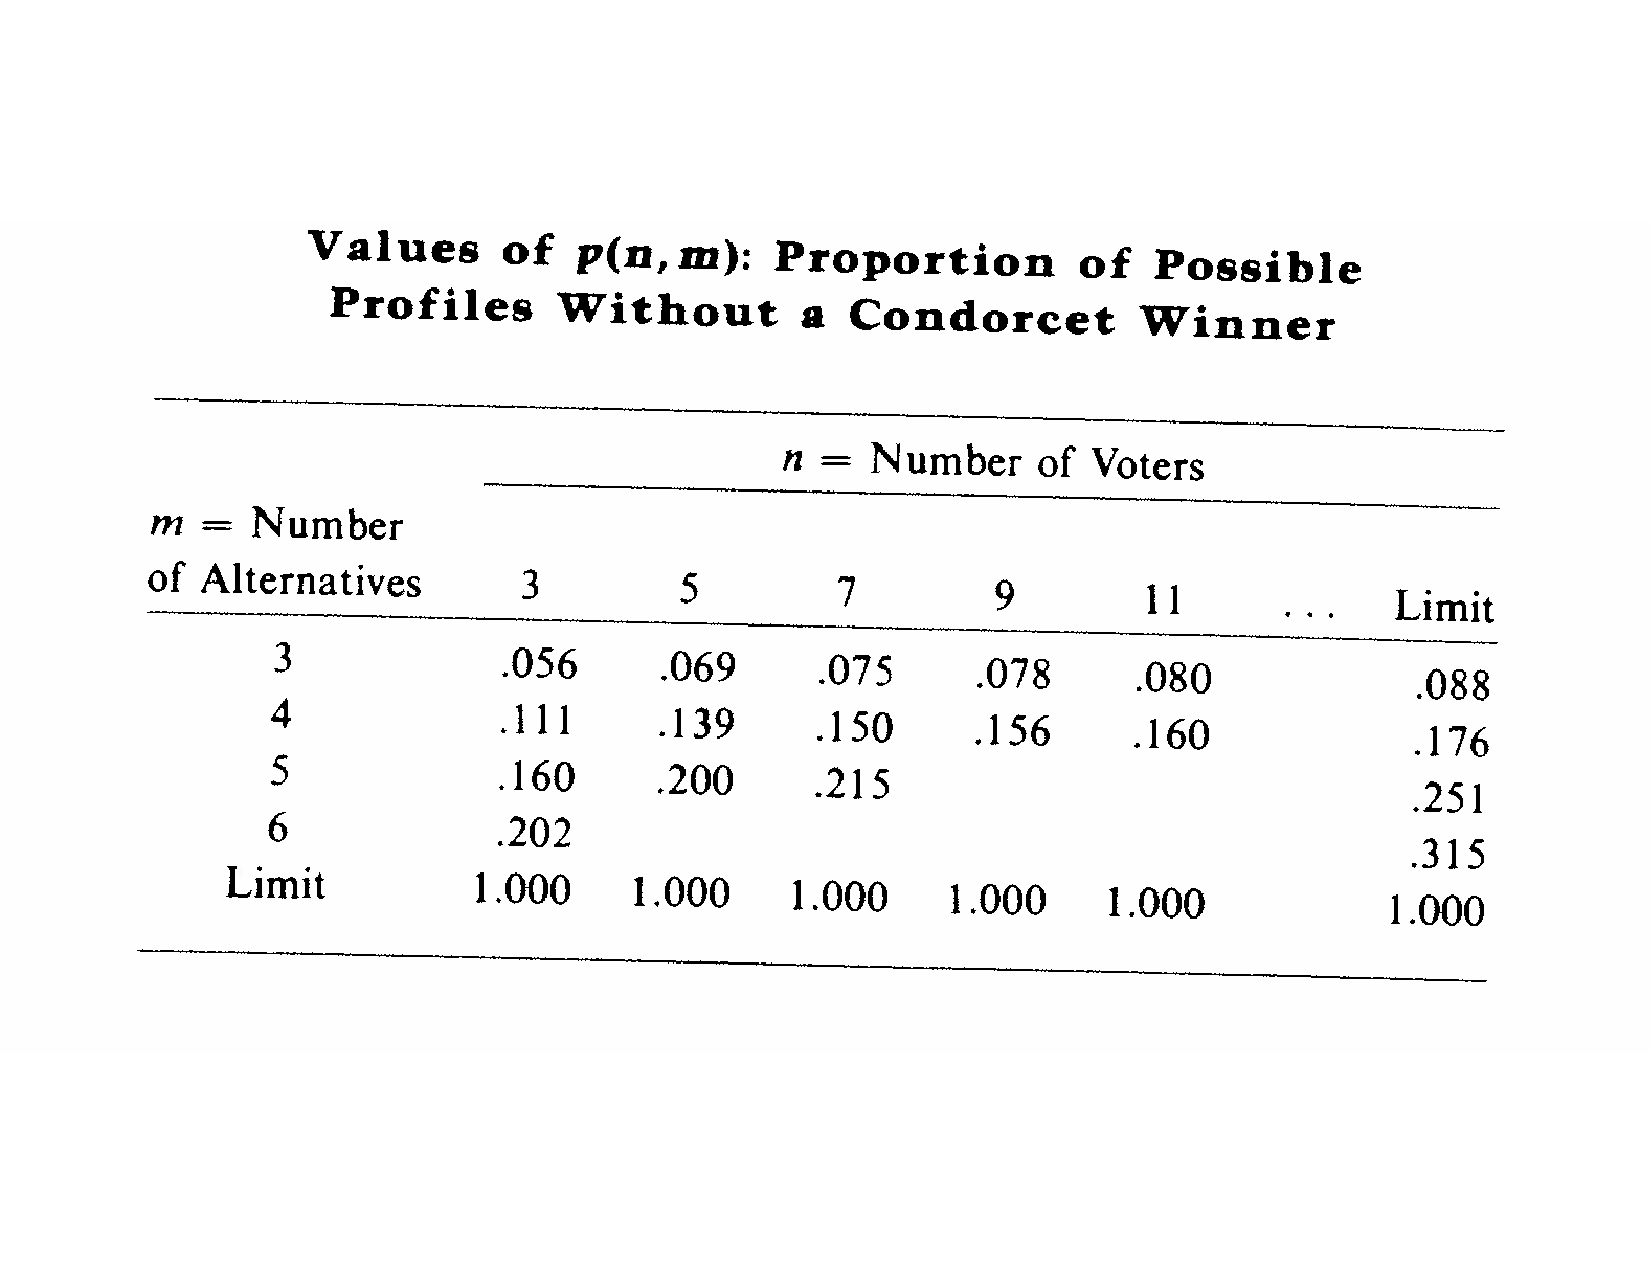
\includegraphics[scale=0.35]{uni2_condorcet1}
    \caption{Probabilidad de ocurrencia de ciclos}
    \label{fig:1}
  \end{figure}
\end{frame}

\begin{frame}\frametitle{¿Qué hacer cuando hay ciclos de Condorcet?}
\begin{itemize}
\item Los ciclos de Condorcet existen, sobre todo, cuando existen
  muchas alternativas entre las cuales elegir y muchos individuos que
  elijen.
\begin{itemize}\itemsep 5pt \medskip
\item ¿existe alguna forma de agregar preferencias que es mejor a otra?
\end{itemize}
\item La respuesta: no existe una respuesta correcta!
\item Ninguna forma es perfecta
\item Este es uno de los resultados mas famosos en la teoría de la
  elección social y se denomina el \textbf{Teorema de la Imposibilidad
    de Arrow}.
\end{itemize}
\end{frame}


% \begin{frame}\frametitle{Ejercitación y práctica}
% \begin{block}{Ordenamiento de preferencias}
% Considere los siguientes perfiles de preferencias para tres
% individuos:
% \begin{enumerate}
% \item $x \succ y \succ z \succ w$
% \item $y \succ z \succ x \succ w$
% \item $z \succ x \succ y \succ w$
% \end{enumerate}
% De acuerdo a la regla de la mayoría, obtenemos que $y \succ z \succ x
% \succ w$. Sin embargo, hay algo que ``está mal'' acercad de este
% ordenamiento social.
% \end{block}
% \end{frame}


\begin{frame}\frametitle{Arrow: el padre de la criatura}
\begin{itemize}
\item Dados:
\begin{itemize}
\item Un conjunto de alternativas, $O$
\item Un conjunto de individuos, $G$
\item Una regla de decisión social, $\succ$
\end{itemize}
\item Las preferencias de un individuo son ``racionales'' si son:
\begin{itemize}\itemsep 5pt \medskip
\item \textbf{Completas} $\longrightarrow$ dadas dos alternativas
  cualquiera, $A$ y $B$, cada individuo puede rankearlas/ordenarlas
  --i.e. $A \succ B$, $A=B$, o $B \succ A$.
\item \textbf{Transitivas} $\longrightarrow$ dadas tres alternativas
  cualquiera, $A$, $B$ y $C$, si $A \succ B$ y $B \succ C$, entonces
  $A \succ C$
\end{itemize}
\end{itemize}
\end{frame}

\begin{frame}\frametitle{El teorema de la imposibilidad: Supuestos}
\begin{itemize}
\item Dominio universal $\longrightarrow$ supone que  individuos
  tienen preferencias racionales sobre cualquier alternativas de $O$
\item Optimalidad de Pareto $\longrightarrow$ si todo los individuos
  de $G$ prefieren $A$ a $B$, la regla de decisión debe
  preferir $A$ a $B$.
\item Independencia de alternativas irrelevantes $\longrightarrow$ si
  hay dos conjuntos de individuos, $G$ y $G'$ y en cada uno sea $A
  \succ B$, el orden entre A y B debe ser el mismo independientemente
  de preferencias por C.
\item No dictadura $\longrightarrow$ ningún $i$ de G tal que sus
  preferencias fijen el orden social independientemente del resto
\end{itemize}
\end{frame}


\begin{frame}\frametitle{Teorema de la imposibilidad}
\begin{block}{Teorema de la imposibilidad de Arrow}
No existe una función de ordenamiento social $\succ$ tal que para
cualquier grupo G cuyos miembros tengan todos preferencias racionales,
$\succ$ sea un ordenamiento racional (transitivo) y que satisfaga los
cuatros supuestos de dominio universal, optimalidad de Pareto,
independencia de alternativas irrelevantes y no dictadura.
\end{block}
\begin{itemize}\itemsep 10pt \medskip
\item Houston, tenemos un problema! $\longrightarrow$ los ciclos de
  Condorcet y el tema del poder de agenda representan problemas
  centrales y fundamentales para los que no hay una solución general.
\item Si queremos una función de ordenamiento social que cumpla con
  todas esas propiedades, no será transitiva $\longrightarrow$ habrá
  ciclos.
\end{itemize}
\end{frame}


\begin{frame}\frametitle{Ejercitación y práctica}
\begin{block}{Ejercicio}
Suponga tres votantes, $G={1,2,3}$. Cada votante tiene un orden
completo de preferencias por tres políticas posibles
$q={q_1,q_2,q_3}$. La política se elige por regla de mayoría
simple. Agenda abierta y voto sincero. Preferencias de los agentes son:
\begin{enumerate}
\item $q_1 \succ q_3 \succ q_2$ ; $q_2 \succ q_1 \succ q_3$  ;  $q_3 \succ q_2 \succ q_1$
\end{enumerate}
\begin{itemize}
\item ¿Existe un ganador de Condorcet? Si votante
  1 fija la agenda (elige rondas de votación con voto
  sincero. ¿Cuál es la agenda óptima según 1?. Si ahora 1 fija la agenda y 2 y
  3 votan sinceramente. ¿Puede el votante 3 mejorar su utilidad
  votando estratégicamente?
\end{itemize}
\end{block}
\end{frame}


\section{Preferencias espaciales y votante mediano}



\begin{frame}\frametitle{Relajando supuestos}
\begin{itemize}
\item Es díficil relajar cualquiera de los supuestos de optimalidad de
  Pareto, independencia de alternativas irrelevantes y de no dictador
  sin caer en injusticias
\item La condición del dominio universal, sin embargo, puede ser
  relajada ya que no es una condición de equidad, sensatez o
  adecuación; es un requisito de dominio.
\item Este es un requisito sumamente restrictivo ya que exige que el
  mecanismo de decisión colectivo funcione en todos los ámbitos
  imaginables (dominio más amplio posible).
\item ¿Que pasa si restringimos el dominio? (menos generalidad)
\end{itemize}
\end{frame}

\begin{frame}\frametitle{Aplicación: Despenalización del aborto}
\begin{itemize} \itemsep 10pt
\item Aborto en EEUU $\longrightarrow$ preferencias polarizadas.
\begin{itemize} \itemsep 5pt \medskip
\item Provida (V) $\longrightarrow$ prohibir aborto bajo cualquier
  circunstancia
\item Proeleccion (E) $\longrightarrow$ mujer derecho absoluto a
  elegir
\item Roe-Wade (1973) (R) $\longrightarrow$
  aborto en etapa temprana
\end{itemize}
\item ¿Cuáles son las preferencias de los grupos?
\begin{itemize}
\item $V \succ R \succ E$ (provida)
\item $E \succ R \succ V$ (proeleccion)
\item $R \succ V \succ E$ (roe-wade1)
\item $R \succ E \succ V$ (roe-wade2)
\end{itemize}
\item Ningun grupo ``extremo'' ni el intermedio considera a $R$ como la peor alternativa
  $\longrightarrow$ ¿consenso?
\end{itemize}
\end{frame}

\begin{frame}\frametitle{Una situación de la vida real (cont.)}
  \begin{figure}[htbp] \vspace{-0.25cm}
    \centering
    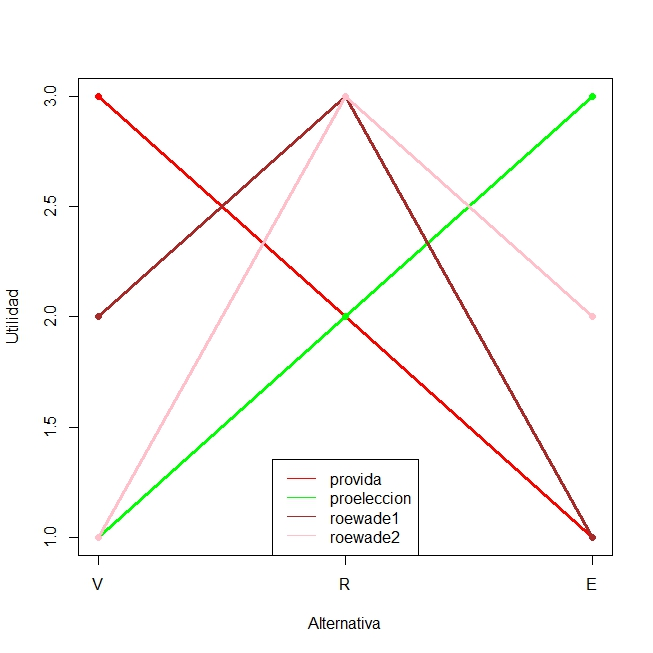
\includegraphics[scale=0.35]{uni2_roewade}
    \caption{Polarización y preferencias de pico único}
    \label{fig:1}
  \end{figure}
\end{frame}

\begin{frame}\frametitle{}
\begin{block}{Teorema del pico único}
Sea un conjunto $O$ de alternativas del cual un grupo $G$ de
individuos debe elegir una. Si, por cada subconjunto de 3
alternativas, y para cada miembro, una de estas \textbf{nunca} es la peor de las tres, entonces el
consenso es lo suficientemente generalizado como para que el método de
la regla de la mayoría arroje preferencias de grupo transitivas
\end{block}
\begin{itemize}\itemsep 10pt
\item Implicancia fundamental $\longrightarrow$ aún si los
  miembros del grupo tienen ideas \textbf{muy diferentes}
  sobre lo que el grupo debería hacer, la \textbf{regla de la mayoría funciona
  a la perfección} siempre y cuando haya un grado mínimo de
  consenso (mediante una curva de pico único).
\end{itemize}
\end{frame}


\begin{frame}\frametitle{Forma de las preferencias}
  \begin{figure}[htbp]
    \centering
    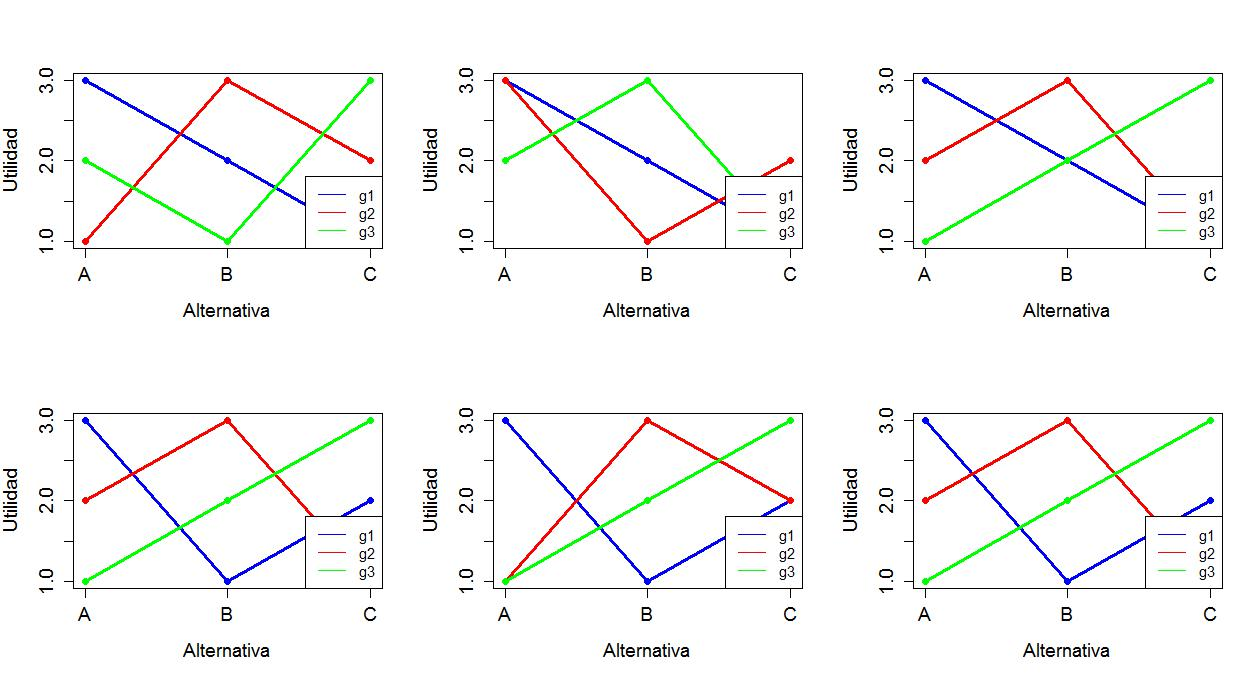
\includegraphics[scale=0.25]{uni2_preferences}
    \caption{Tipología de preferencias individuales}
    \label{fig:1}
  \end{figure}
\end{frame}

\begin{frame}\frametitle{Restricción de dominio: preferencias}
\begin{itemize}\itemsep 10pt
\item Si las preferencias son de pico único,
  entonces la regla de la mayoría produce una agregación de
  preferencias individuales a sociales que cumple todas las
  condiciones de Arrow y que además es transitiva.
\item ¿Es razonable restringir las preferencias de este
  modo?
\begin{block}{Preferencias en la práctica}
Suponga 3 partidos: izquierda (I), centro (C), y derecha
(D). El individuo 1 se identifica con I. Tendrá $I \succ C
\succ D$. El individuo 2 se identifica con D y tendrá $D \succ C \succ I$. Y el de centro podrá tener $C \succ
\ D \succ I$ o $C \succ I \succ D$.
\end{block}
\end{itemize}
\end{frame}

\begin{frame}\frametitle{Ejemplos de preferencias de pico único}
\begin{itemize}\itemsep 10pt
\item Pueden pensarse las preferencias de ciudadanos por diferentes
  asuntos:
\begin{itemize}\itemsep 5pt \medskip
\item Preferencias escala ideológica liberalismo-conservadurismo
\item Preferencias por tasa impositiva y gasto público en educación
\item Preferencias por localización de bien público (plaza)
\item Preferencias por arancel a importación
\end{itemize}
\item En cualquier caso, una función de utilidad que describe
  preferencias de tipo único es del tipo ($b_i$ es el punto ideal del
  individuo $i$):
\end{itemize}
\begin{align*}
u_i=-(g-b_i)^2  \\
u_i=1-\lvert g-b_i \rvert
\end{align*}
\end{frame}


\begin{frame}\frametitle{Ejemplos de preferencias de pico único (cont.)}
 \begin{figure}[htbp]
    \centering
    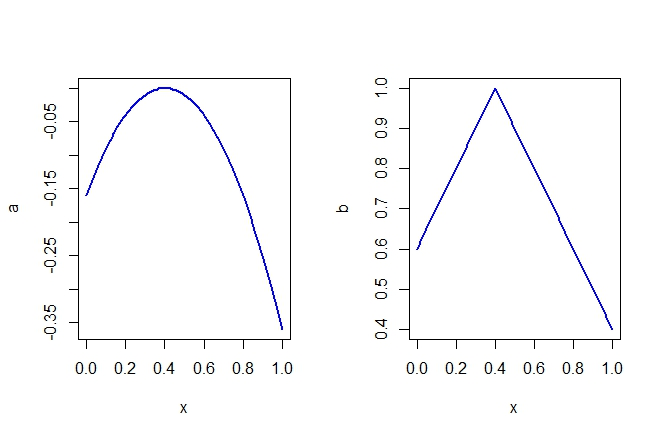
\includegraphics[scale=0.4]{uni2_utility1}
    \caption{Funciones de utilidad de pico único}
    \label{fig:1}
  \end{figure}
\end{frame}


\begin{frame}\frametitle{Preferencias sociales: de pico
    único?}
\begin{itemize}\itemsep 15pt
\item Se ha criticado la restricción de las preferencias a las de pico
  único argumentando que no aplican a muchas situaciones
  económicas y políticas
\item Muchos problemas económicos   --alícuotas impositivas; tamaño del gobierno; gasto en defensa;
  localización de un bien público- son variables continuas que pueden
  modelarse con preferencias de pico único.
\item El problema surge con elecciones entre cosas
  que no tienen un orden dado --qué banda debería tocar en un evento;
  de qué color pintar las aulas. 
\end{itemize}
\end{frame}


\begin{frame}\frametitle{Preferencias en el espacio}
\begin{itemize}\itemsep 10pt
\item Problema del grupo $\longrightarrow$ escoger un punto de una
  línea.
\end{itemize}
\begin{block}{Problema del directorio}
La junta de directores del BCRA deben adoptar una decisión sobre la
tasa de interés interbancaria. Las tasas de interés, en cuanto
números, son en efecto puntos de una línea: el extremo inferior es
0\%, el extremo superior 10\%, es decir la linea se traza para el
intervalo [0,10]. Supongamos que hay 5 (cinco) directores y que cada
uno tiene un punto de esa linea (tasa) que es el que más desea y luego
sus preferencias disminuyen a medida que se alejan de ese punto en
cualquier dirección
\end{block}
\end{frame}

\begin{frame}\frametitle{Preferencias en el espacio (cont.)}
 \begin{figure}[htbp]
    \centering
    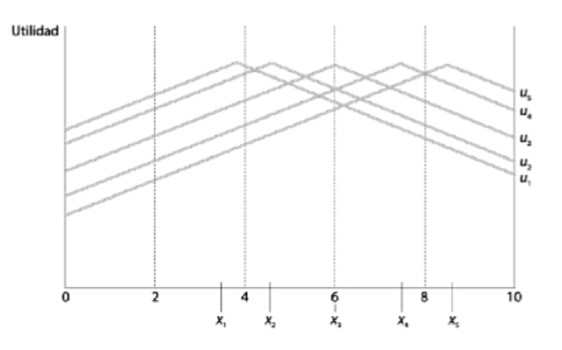
\includegraphics[scale=0.5]{uni2_tvm5}
    \caption{Preferencias a lo largo de una linea}
    \label{fig:1}
  \end{figure}
\end{frame}


\begin{frame}\frametitle{Preferencias en el espacio (cont.)}
\begin{itemize}\itemsep 10pt
\item Las cinco personas, $G={1,2,3,4,5}$ tienen las preferencias
  mostradas en el gráfico anterior y representadas como
  $x={x_1,x_2,x_3,x_4,x_5}$.
\item Cada individuo tiene un punto favorito $\longrightarrow$ ``punto
  ideal''. Esa es la tasa de interés que el/ella prefiere en primer
  lugar. Por ejemplo, para el director 1:
\begin{itemize}\itemsep 5pt
\item $x_1 \succ x_2 \succ x_3 \succ x_4 \succ x_5$
\end{itemize}
\item Las preferencias se ``miden'' a partir de la utilidad --i.e. la
  altura de la curva; cada una de las ``campanas'' es una función de
  utilidad para cada director.
\end{itemize}
\end{frame}

\begin{frame}\frametitle{Preferencias en el espacio (cont.)}
 \begin{figure}[htbp]
    \centering
    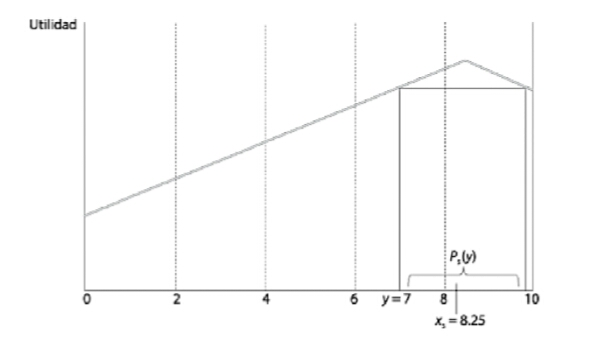
\includegraphics[scale=0.43]{uni2_tvm6}
    \caption{Conjuntos preferidos}
    \label{fig:1}
  \end{figure}
\end{frame}


\begin{frame}\frametitle{Preferencias en el espacio (cont.)}
\begin{itemize}\itemsep 10pt
\item Tomemos ahora solamente al individuo 5. Su perfil de
  preferencias es $x_5 \succ x_4 \succ x_3 \succ x_2 \succ x_1$. Su
  tasa de interés favorita (punto ideal) es de $8.25$.
\item Tomemos una tasa cualquiera --i.e. $7$. El conjunto de puntos
  (tasas) que este individuo prefiere a $7$ es el que se representa
  como $P_5(y)$: ese conjunto contiene a todas las tasas de interés
  entre 7 y 9.25 [¿Por qué?]
\item En otras palabras, si la tasa $y$ fuera una propuesta concreta,
  este individuo prefería todos los puntos del conjunto $P_5(y)$ a $y$.
\end{itemize}
\end{frame}

\begin{frame}\frametitle{Preferencias en el espacio (cont.)}
 \begin{figure}[htbp]
    \centering
    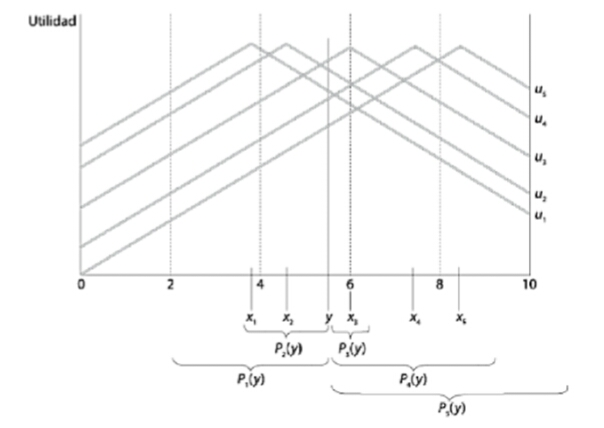
\includegraphics[scale=0.40]{uni2_tvm7}
    \caption{Superponiendo los conjuntos preferidos}
    \label{fig:1}
  \end{figure}
\end{frame}

\begin{frame}\frametitle{Preferencias en el espacio (cont.)}
\begin{itemize}\itemsep 10pt
\item Ahora veamos los ``conjuntos preferidos a $y$'' de todos los
  directores (note $y$ un poco abajo de $6$). Puede verse que:
\begin{itemize}\itemsep 5pt \medskip
\item $P_4(y)$ y $P_5(y)$ tienen puntos en común
\item $P_1(y)$ y $P_2(y)$ tienen puntos en común
\item Los individuos 3, 4 y 5 tienen conjuntos preferidos a $y$ que se
  superponen; estos tres individuos forman una mayoría (3 contra 2)
  por lo que esa mayoría vence a una propuesta como $y$.
\end{itemize}
\item Pueden pensarse en todas las mayorías posibles que vencen a
  $y$ dependiendo de posición de $y$ en la escala.
\item Coaliciones de mayorías posibles
  que vencen a $y$.
\end{itemize}
\end{frame}


\begin{frame}\frametitle{Preferencias y coaliciones}
  \begin{table}[htbp]
    \centering
    \begin{tabular}[htbp]{|c|p{5cm}|} \hline
      Tamaño coalicion & Coalicion \\ \hline
3 & (1,2,3) (1,2,4) (1,2,5) (1,3,4) (1,3,5) (1,4,5) (2,3,4) (2,3,5)
    (2,4,5) (3,4,5) \\\hline
4 & (1,2,3,4) (1,2,3,5) (1,2,4,5) (1,3,4,5) (2,3,4,5) \\\hline
5 & (1,2,3,4,5) \\\hline
    \end{tabular}
    \caption{Coaliciones de mayorias}
    \label{tab:1}
  \end{table}
\end{frame}


\begin{frame}\frametitle{El rol del mediano}
\begin{figure}[htbp]
    \centering
    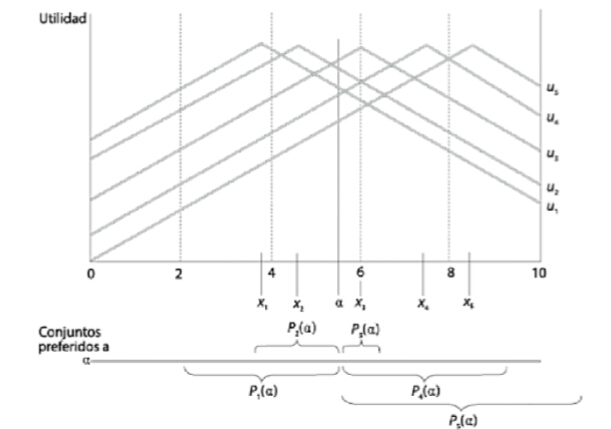
\includegraphics[scale=0.40]{uni2_tvm8}
    \caption{El rol del votante mediano}
    \label{fig:1}
  \end{figure}
\end{frame}

\begin{frame}\frametitle{El rol del mediano (cont.)}
\begin{block}{Teorema del votante mediano (TVM)}
Si miembros de un grupo $G$ tienen preferencias de pico único, el punto ideal del VM es un ganador de Condorcet.
\end{block}
\begin{itemize}\itemsep 10pt
\item Sería $x_3$. Suponga $\alpha$ a
  la izquierda de $x_3$. Miembros 1 y 2 prefieren $\alpha$ pero 3,
  4 y 5 prefieren $x_3$ a $\alpha$.
  $x_3$.
\item Suponga $\beta$ a la derecha de $x_3$. Miembros 4 y 5 pueden preferirlo a $x_3$ pero los miembros 1, 2 y 3
  prefieren $x_3$ a $\alpha$.
\item $x_3$ vence a todos los puntos restantes. El punto ideal del
  VM no es vencido por ninguno y esta es la decisión de mayoría.
\end{itemize}
\end{frame}


\begin{frame}
\frametitle{El teorema del votante mediano}
\begin{itemize}
\item El teorema postula que hay un único ganador por mayoría y que ese ganador es el VM --aquel  el medio de la distribución en relación a la dimensión explorada
\item Uno de los resultados más importantes en la
  teoría de la votación $\longrightarrow$ postula una convergencia a
  las preferencias del votante mediano.
\begin{itemize}\itemsep 5pt \medskip
\item En cualquier situación de elección en votación por mayoría, la
  mejor forma de obtener la mayoría de los votos es acercarse a las
  preferencias del votante mediano.
\end{itemize}
\item El TVM no aplicable a situaciones de más de dos dimensiones de las preferencias $\longrightarrow$ originan ciclos 
\end{itemize}
\end{frame}


\begin{frame}\frametitle{El teorema del votante mediano (cont.)}
\begin{itemize}
\item Note que la \textit{intensidad de las preferencias} no importa
  para nada en este resultado.
\begin{itemize}\itemsep 5pt \medskip
\item Puede que me desagrade mucho un candidato pero mi voto cuenta
  exactamente lo mismo que el de otra persona que es casi indiferente
  entre ese candidato y cualquier otro.
\end{itemize}
\item Se deriva del principio ``una persona, un voto''
  $\longrightarrow$ una de las diferencias fundamentales entre las
  elecciones y las decisiones económicas
\begin{itemize} \itemsep 5pt \medskip
\item Se puede relajar esto (volveremos mas adelante)
  $\longrightarrow$ costo de votar (registración); contribuciones de
  campaña; influencia.
\end{itemize}
\end{itemize}
\end{frame}

\begin{frame}
\frametitle{El teorema del votante mediano (cont.)}
% \begin{center}
% \begin{figure}
% \begin{pspicture}(0,0)(8,4)
% \psaxes[ticks=none,labels=none,linewidth=0.5pt]{<->}(0,0)(0,0)(8,4)
% \psarc[linecolor=blue,linewidth=0.04](1.50,1.2){1}{0.0}{180.0}
% \psarc[linecolor=blue,linewidth=0.04](3.20,0.8){1}{0.0}{180.0}
% \psarc[linecolor=blue,linewidth=0.04](5.4,0.4){1}{0.0}{180.0}
% \psline[linestyle=dashed,linecolor=blue,linewidth=0.02cm](1.50,2.14)(1.5,0)
% \psline[linestyle=dashed,linecolor=blue,linewidth=0.02cm](3.2,1.78)(3.2,0)
% \psline[linestyle=dashed,linecolor=blue,linewidth=0.02cm](5.4,1.32)(5.4,0)
% \rput(-0.3,3.8){$u_{i}$}
% \rput(8.4,0){$p$,$\pi$}
% \rput(5.4,-0.3){$x_{3}$}
% \rput(3.2,-0.3){$x_{2}$}
% \rput(1.5,-0.3){$x_{1}$}
% \rput(0.5,1.05){$i=l$}
% \rput(2.28,0.62){$i=m$}
% \rput(4.4,0.25){$i=r$}
% \rput(0.5,-0.3){$x_{min}$}
% \rput(6.7,-0.3){$x_{max}$}
% \psdot(0.5,0)
% \psdot(1.5,0)
% \psdot(3.2,0)
% \psdot(5.4,0)
% \psdot(6.7,0)
% \end{pspicture} \bigskip
% \caption{Teorema del votante mediano: Ordenamiento de preferencias
%   individuales (preferencias de pico único)}
% \end{figure}
% \end{center}

\begin{figure}[htbp]\vspace{-0.3cm}
  \centering
  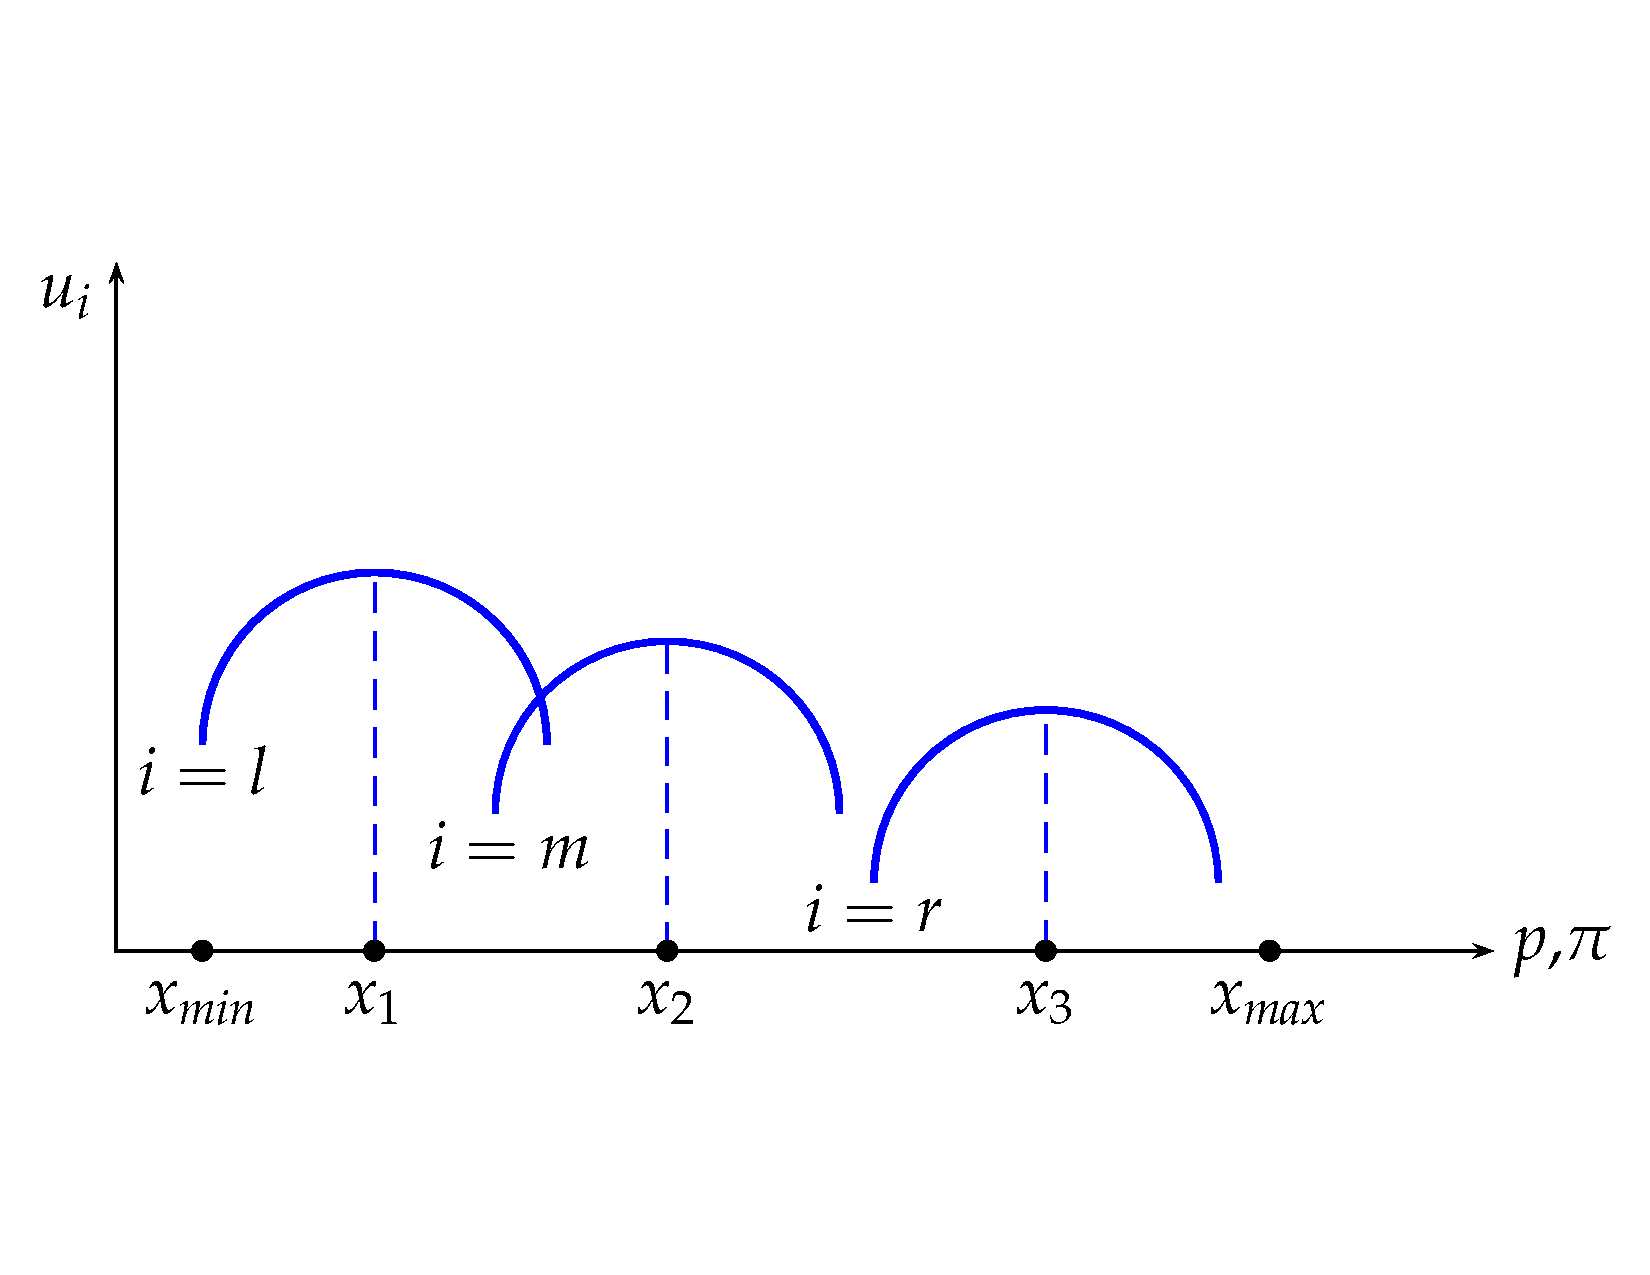
\includegraphics[scale=0.3]{uni2_tvm1}
  \caption{Teorema del votante mediano: Ordenamiento de preferencias
    individuales (preferencias de pico único)}
  \label{fig:3}
\end{figure}
\end{frame}


\begin{frame}\frametitle{Supuestos restrictivos del análisis}
\begin{itemize}
\item Estos ejemplos y razonamientos se basan en 3 (tres) supuestos
  implícitos:
\begin{itemize}\itemsep 5pt \medskip
\item Número impar de miembros $\longrightarrow$ el mediano es el que
  está siempre en el medio de la distribución (espacial). Si el número
  de miembros fuera par (por ejemplo, 4), tanto 2 y 3 son medianas. Es
  decir, habria ganadores de Condorcet, pero no serían únicos.
\item Participación total $\longrightarrow$ todos votan. No siempre
  pasa en la práctica (abstenciones, ausencias, etc). El resultado del
  votante mediano se aplica pero cambia la identidad del votante
  mediano --i.e. cambia el punto elegido.
\item Voto sincero $\longrightarrow$ si las personas no votan de
  acuerdo a sus preferencias (voto sincero), entonces existe voto
  estratégico. Esto cambia de forma importante los resultados.
\end{itemize}
\end{itemize}
\end{frame}


\begin{frame}\frametitle{Limitaciones centrales}
\begin{itemize}
\item Algunas limitaciones de este modelo son:
\begin{itemize}\itemsep 5pt \medskip
\item Son modelos de decisión colectiva
  \textbf{unidimensionales}. Muchísimas situaciones sociales en que la
  cuestión no puede reducirse a una sola dimensión.
\item Voto a presidente/gobernador $\longrightarrow$ dimensión
  económica y dimensión social.
\item Elección en concursos de cantantes, belleza --i.e. varias dimensiones
\end{itemize}
\item Cuando se generaliza a mas de una dimensión, el resultado del
  votante mediano es mucho más restrictivo.
\item No da ningún rol a las instituciones políticas 
\end{itemize}
\end{frame}


\begin{frame}\frametitle{Ejercitación y práctica}
\begin{block}{Ejercicio}
Suponga tres opciones de restaurant:
\begin{itemize}
\item $A$ cuesta 5 dolares
\item $B$ cuesta 10 dolares
\item $C$ cuesta 20 dolares
\end{itemize}
Hay tres personas $G={1,2,3}$. La persona 1 prefiere $A$; la persona 2
prefiere $B$ y la persona 3 prefiere $C$.
\begin{itemize}
\item ¿Qué implican las preferencias de pico único en este caso?
\item ¿Qué restaurante es elegido? ¿Por qué?
\end{itemize}
\end{block}
\end{frame}

\end{document}


